\subsection{Cyclic \suldiox~Hydrate Structures}

Having examined the bonding coordinations and bonding behavior of \suldiox~with surface waters, we now turn to a secondary behavior of the hydrate structures that form around the surface-bound \suldiox~molecule. The simulation trajectory data was analyzed to determine the presence and characteristics of \suldiox~cyclic hydrate structures that form during MD, as posited earlier and depicted in Figure \ref{fig:cyclic-structures}. Only the most commonly occurring subset of the cyclic structures were analyzed. 

\begin{figure}[h!]
	\begin{center}
		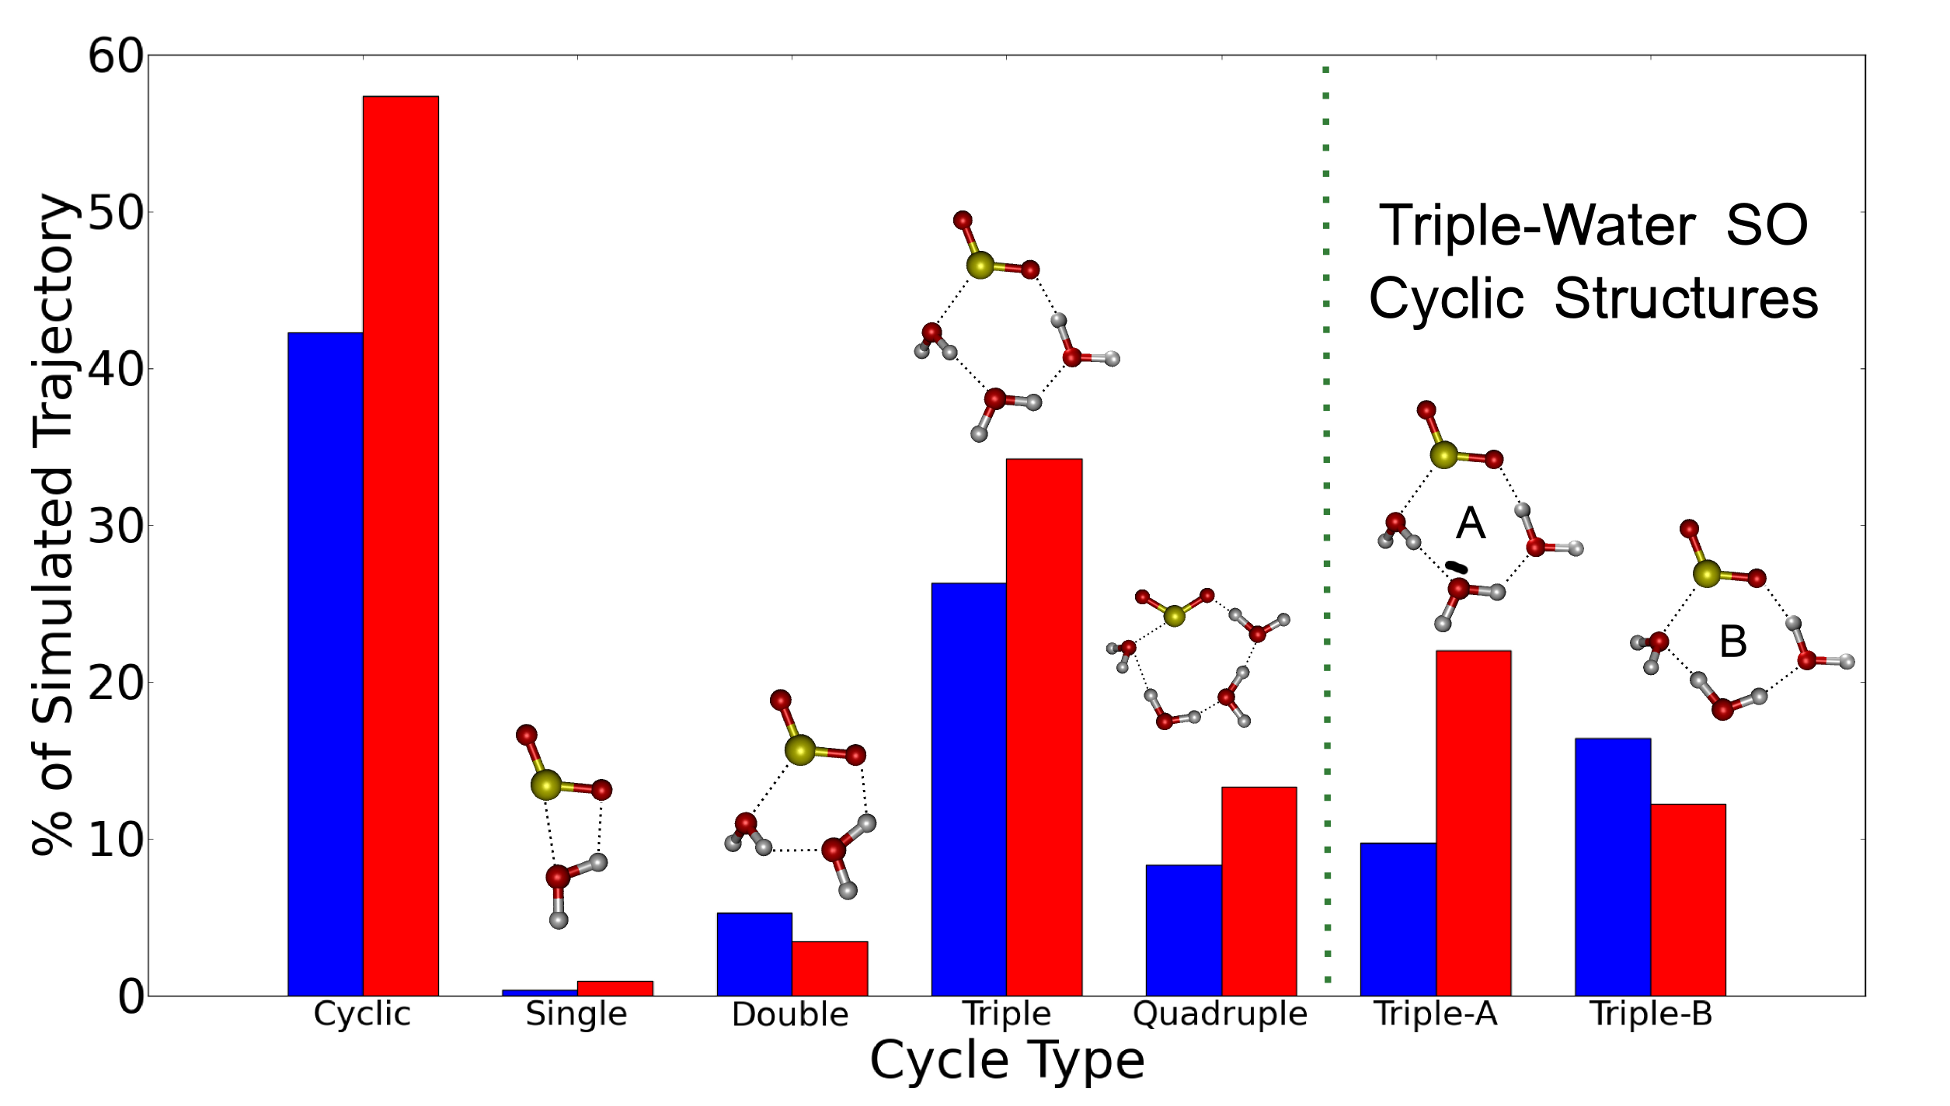
\includegraphics[scale=1.0]{images/cycles/SO-cycle-breakdown-with-cartoons-small.png}
		\caption{}
		\label{fig:cyclic-breakdown}
	\end{center}
\end{figure}
The plot in Figure \ref{fig:cyclic-breakdown} shows the distribution of how often the various types of cyclic hydrates were encountered at both cold (blue) and hot (red) temperatures. Each data point shows a percentage of the MD trajectories in which the \suldiox~was a member of a cyclic structure, for different numbers of cyclic waters (up to 4). The two tallest data points, left-most in the plot, show the overall time spent in all types of cyclic structures. Clearly the hot system \suldiox~spends more time in a cyclic structure than at the cold temperature. The plot is based on two criteria for determining if a cyclic structure has formed. (1) The distances between atoms must match the same bonding/distance criteria as used for determining bonding coordinations. (2) The \suldiox~must be minimally in a bonding coordination of type ``SO'', meaning that the sulfur has at least one bonding interaction, and at least one hydrogen-bond must have formed with an oxygen to a neighboring water-hydrogen. As noted earlier in the discussion of the graph-finding routine and the BFS algorithm, the cyclic structures found represent the smallest cycles in which the \suldiox~is a member, based on order of discovery. The \suldiox~will be inevitably involved in other larger and more extended cyclic bonding structures beyond the first one discovered via the BFS. The larger and more extended cyclic structures involving more waters affect the behavior of the hydrogen-bonding network of the water surface. However, we focus here only on the smallest cycles involving the \suldiox~as the most affect the \suldiox~bonding and hydrating behaviors.

It is remarkable that the difference of the time spent in a cyclic structure between the two temperatures is 15\% (42\% cold, 57\%hot). The hot \suldiox~spends well over half of the simulated time bound as one of the hydrate cycles, and the cold \suldiox~spends just under half of the time as such. Thus, in addition to having found the most likely bonding coordination during the simulated life of \suldiox, we have also found that the hydrates of the \suldiox~form a cyclic structure for much of the time it is bound to the water surface.

Now we look at the different types of cyclic hydrates, distinguished by the number of waters involved in the bonding structure. In Figure \ref{fig:cyclic-breakdown} the single and double water cycles are the least frequently encountered structures, accounting for less than 10\% of both temperature simulations. Formation of the single type is likely energetically unfavorable because of the proximity of the single water to the \suldiox. The double-water structure was one of two types of clusters proposed in a previous computational work as a candidate structure contributing to the overall IR spectrum of surface-bound \suldiox.\cite{Baer2010} In the static and geometry-optimized cluster calculations, lacking the extended water structure or bonding from waters external to the hydrate, both the double and triple types appear equally likely to form. However, the MD simulations here have introduced many waters into a dynamic environment allowing for extended bonding networks, and the results show clearly that the double-water cyclic hydrate is formed much less often (less than 5\% at both temperatures) than the triple-water form.

The results for triple and quadruple-water structures show that larger hydrate cycles are favored at higher temperatures. Although the higher number of hydrating waters (>4) are not shown, those contribute minimally to the overall distribution. The majority of the cyclic hydrates are formed with three waters in the triple type. This hydrate type matches the bonding structure inferred from our previous experiments, and also one of the cluster types modeled by others.\cite{Tarbuck2005,Tarbuck2006,Baer2010} It was further found that of the triple-type hydrate cycles, the waters contributing to the cycles can be arranged in two ways that preserve the hydrogen-bonding between the molecules. The two triple cycle structure are depicted on the right side of Figure \ref{fig:cyclic-breakdown}, along with the plots of the contributions to the overall distribution. It is notable that each temperature has a different dominant type of triple-water cyclic structure. The cold system forms more of the type-B, and the hotter system forms primarily triple type-A.

\subsection {Cyclic Structure Energy Calculations}

\subsection {Cyclic Hydrate Structure Lifetimes}

Knowing that the \suldiox~bound to a water surface is most likely in the ``SO'' bonding coordination, and also often taking part in some type of cyclic structure, how long does the cyclic hydrate form before breaking to an acyclic structure? To answer the questions of cyclic lifespans, a method was devised to define a lifetime of a cycle. For each trajectory, the coordinate data was analyzed to determine if a cyclic hydrate structure was formed based on the bonding distance criteria established earlier in this manuscript. A timeline was then produced where each timestep was given a value of 1 or 0 if a \suldiox~cycle was found or not found, respectively. This resulted in a time-function, $C(t)$, similar in nature to a digital signal. The resulting cycle formation time-function is plotted for one of the simulated trajectories shown as the dashed black line in Figure \ref{fig:debouncing}. At the far left of the plot the function is in the ``no cycle'' state, and then switches ``on'' as a cycle is formed. The cyclic structure is very dynamic constantly moving and distorting, so any of the bonds forming the cyclic bonding structure are liable to break and reform quickly. This is manifested in Figure \ref{fig:debouncing} as a series of very sharp spikes in the function lasting less than 10 fs each. Because of the very rapid breaking and reformation of the cyclic structure, a procedure was used to ``debounce'' the time-function to disregard very brief moments when the cycle breaks or forms for less than 20 fs. The time-function, $C(t)$ was smoothed using a moving gaussian window function with a 10 fs width. The resulting smoothed function, $C_s(t)$, was then cutoff with the following criteria:

\[
  f(t) = \left\{ 
  \begin{array}{l l}
    0 & \quad C_s(t) < 0.2\\
    1 & \quad C_s(t) \geq 0.2\\
  \end{array} \right.
\]

where $f(t)$ is the debounced time-function that better represents the lifespans of cycles, eliminating the very brief discontinuities and excursions outside the bonding criteria that cause the rapid ``bouncing'' of the cyclic time-function, $C(t)$. Figure \ref{fig:debouncing} shows the original time-function of cycle formation and breaking, $C(t)$ (dashed black), the smoothed function, $C_s(t)$ (red), and the final ``debounced'' function, $f(t)$ (green).

\begin{figure}[h!]
	\begin{center}
		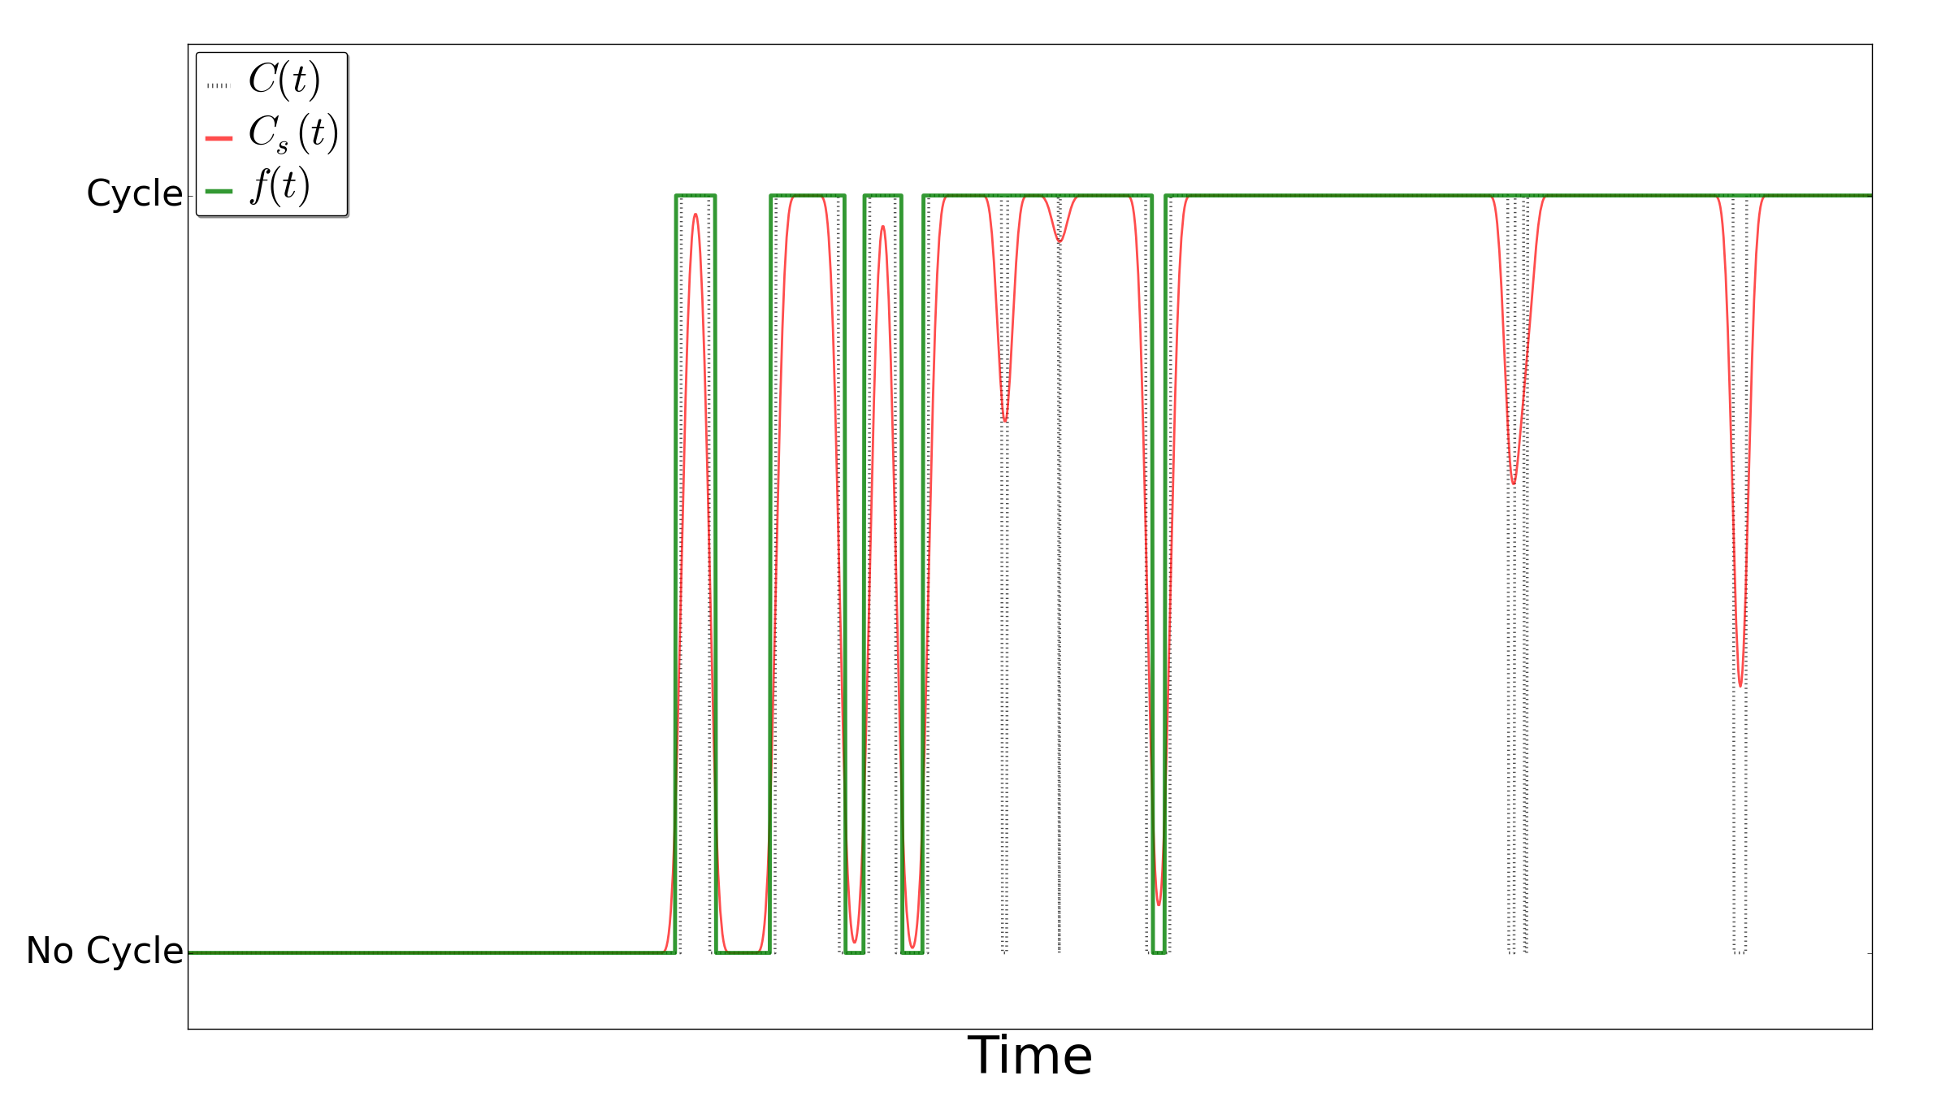
\includegraphics[scale=1.0]{images/cycles/cycle-debouncing-small.png}
		\caption{}
		\label{fig:debouncing}
	\end{center}
\end{figure}

The distribution of cycle lifetimes (i.e. contiguous spans of time spent with $f(t) = 1$) was determined. A plot of the cyclic lifespans is shown in Figure \ref{fig:cycle-lifespans} for the cold (blue) and hot (red) simulations. The most frequent lifespan for both temperature data sets lasts between 0-1 ps. This accounts for the vast majority of cyclic hydrates found (approximately 95\%) indicating that these structures are very transient, and are continuously forming and breaking for very short periods of time. Even with the ``debouncing'' procedure that would artificially increase the timespan spent either formed or broken, the nature of the water surface, and the very dynamic extended hydrogen bonding network, keeps many of the structures from lasting much longer than 1 ps. The difference between hot and cold systems in the $<1$ ps population is less than 2\%, with this trend also extending to the longer lifespans as well. The inset of figure \ref{fig:cycle-lifespans} shows an expanded view of the region above 1 ps. All of the distribution shows only a $<1.5$\% difference between cold and hot cyclic lifetimes. Overall, the distribution shows that when cycles form, at both temperatures, they last a similar amount of time. 

Up to 3 ps, the cold temperature cycles show a very slight population increase above the hot temperature cycles. Above 4 ps, most of the cycles that form are found in the hot system. The 8 ps cycles are notable in that they form  for just under half of an entire single simulated trajectory.

We know from the transition frequency plots of Figure \ref{fig:coordination-transitions} that the bonding coordinations are switching frequently. The \suldiox~is likely forming and breaking bonds with waters extraneous to the cyclic hydrate structures (i.e. not directly involved in the bonds of the cycle). For the longer-lived cycles, the extraneous bonding to the \suldiox~may have little effect on the cyclic hydrate waters. However, any time the \suldiox~switches into an unbound, sulfur-only, or oxygen-only coordination (i.e. ``S'', ``SS'', ``O'', etc), the cyclic structure is necessarily broken. Because the majority of cyclic structures last only briefly ($<1$ ps), the active switching of \suldiox~bonding coordinations appears to break the cyclic structure. Figure \ref{fig:bonding-coordinations} shows the sum of coordinations that necessarily break cyclic structures account for approximately 39\% and 24\% of the bonding coordinations in the cold and hot system, respectively. Consequently, the distribution of Figure \ref{fig:cyclic-breakdown} also indicates that there are more cycles formed in the hot system (approximately 16\% above the cold). The increased temperature appears to cause the \suldiox~to bond in such a way that is more conducive to the formation of cyclic structures. Furthermore, the distribution of bonding coordinations in the hot system shifts the transition between bonding coordinations away from cycle-breaking coordinations (i.e. those coordinations that necessarily disallow cycle formation). This possibly accounts for the slightly increased populations of longer cycle lifespans in the hot system (greater than 4 ps in some cases) compared to the cold system in the cycle lifespan distribution of Figure \ref{fig:cycle-lifespans}. 

\begin{figure}[h!]
	\begin{center}
		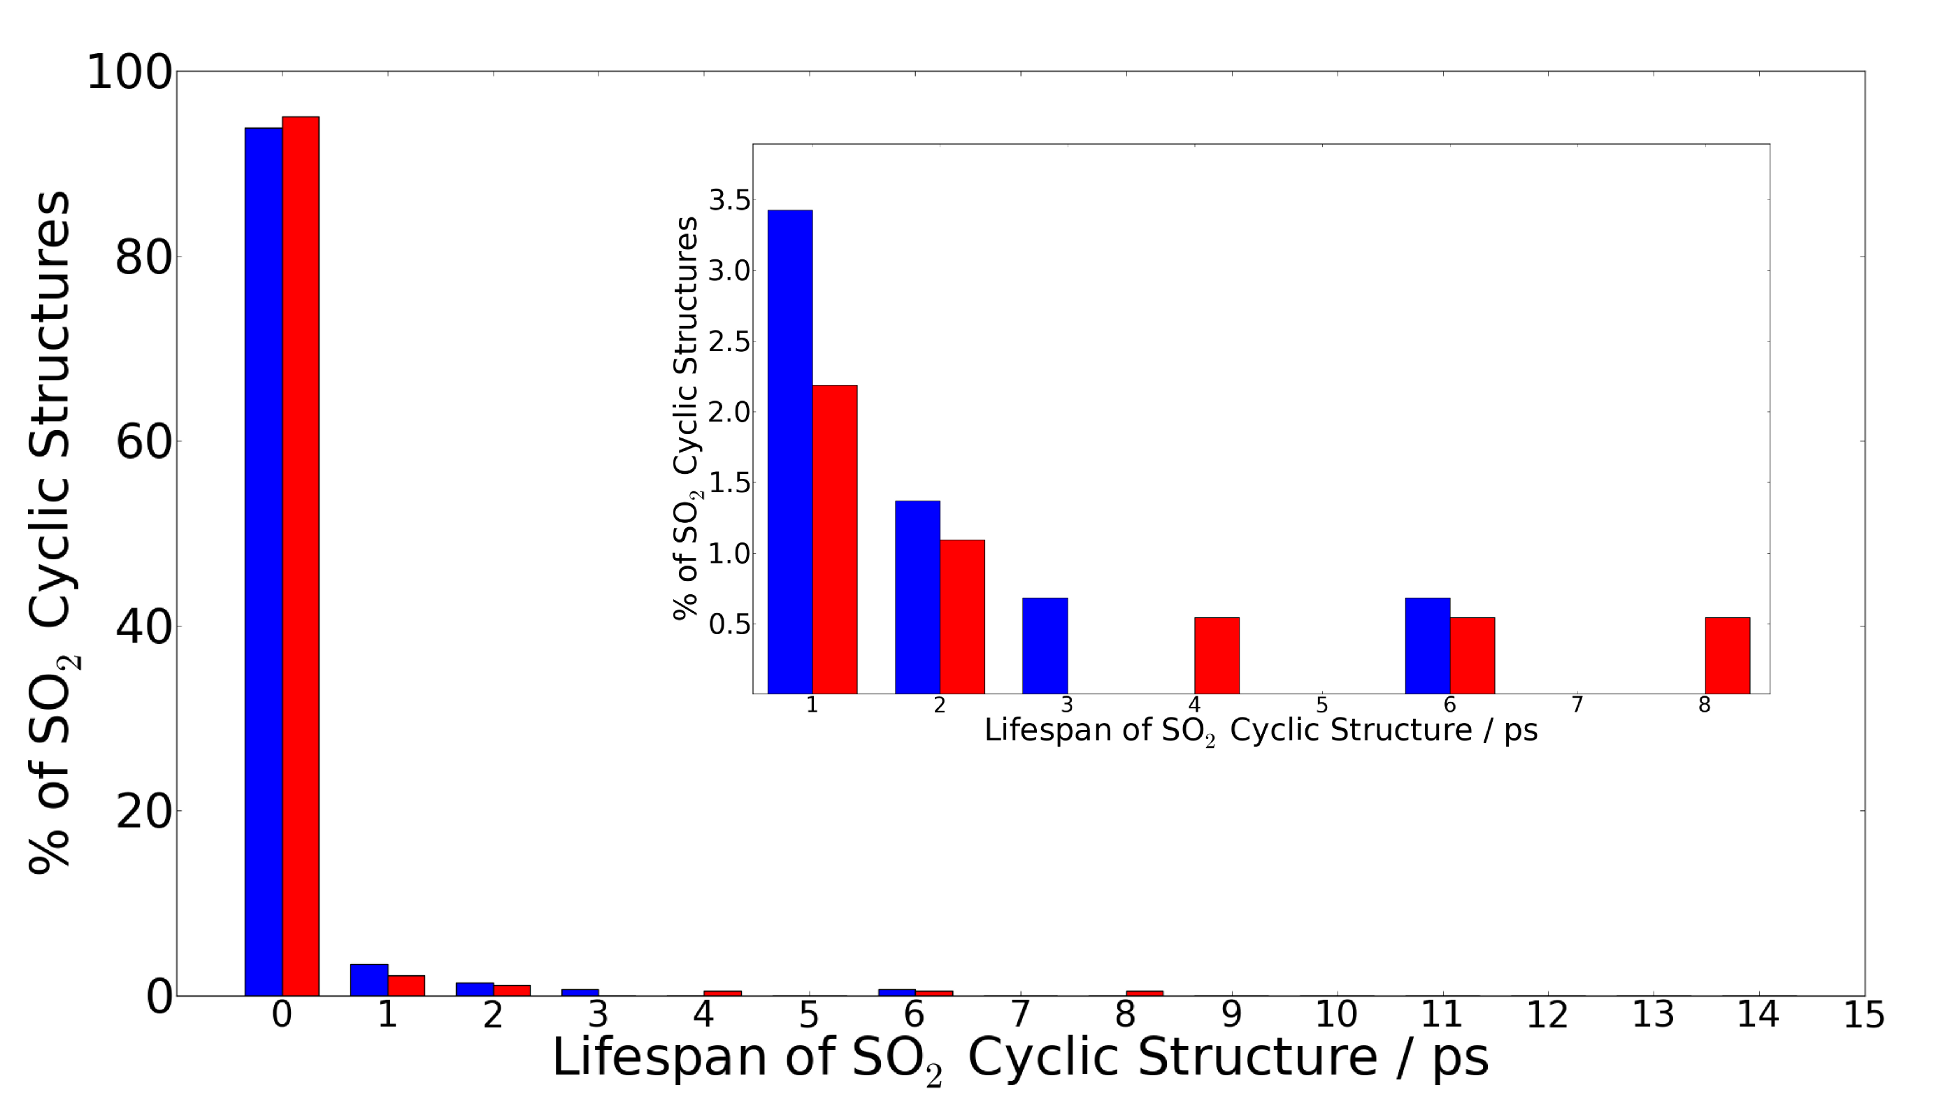
\includegraphics[scale=1.0]{images/cycles/cyclic-lifespans-inset-small.png}
		\caption{}
		\label{fig:cycle-lifespans}
	\end{center}
\end{figure}
